\chapter{Direct Data-Driven Control design}
\section{introduction}

In this chapter a new approach for designing controllers is going to be adopted. In general for designing controllers we have the following situations:
\begin{itemize}
    \item \textbf{Model-based controller design}: in this case, the model of the system is known and is used to design the controller in a convensional manner.
    
    \item \textbf{Data-Drive controller design}: here, the model of the system is obtained using experimental data, by means of SM identification for instance. Afterwards, the model is used in order to design the controller.
    
    \item \textbf{Direct Data-Driven controller design}: In this method, there is no need for an intermediate step of identifying the model of the system. In this appraoch, the controller is designed without knowing the model of the system and just by using the experimental input-output data.
    
\end{itemize}

In this chapter the third case is going to be discussed. The scheme we considere here is as follows: 
 \begin{figure}[H]
    \centering
    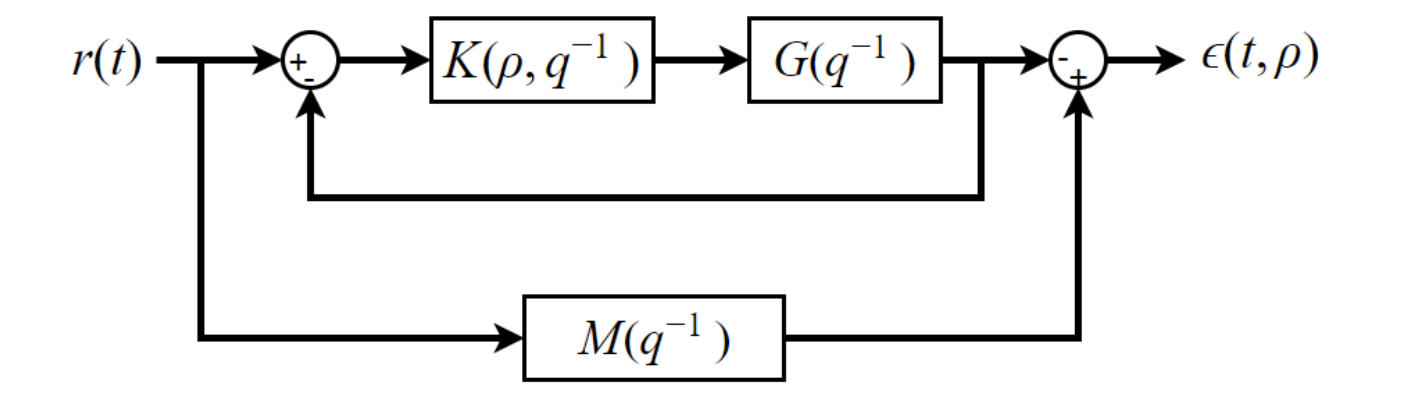
\includegraphics[width=0.75\textwidth]{dddc-scheme.png}
    \caption{Feedback control system to be designed compared with the
 reference model $M(q^{-1})$}
 \end{figure}
In this scheme, $M$ represents the \textbf{reference model}, the resultant control system, which is expected to satisfy the requirements, and $G$ is the unknown plant to be controled. 


\section{DDDC design procedure}
\subsection{Task 1: to find the controller}
The first task is to find a controller $K(\rho,\,q^{-1})$ - $K$ is an LTI discrete-time system with a transfer function depending on some parameter $\rho$ - such that the complementary sensitivity function of the controller,$T$, is close enough to the transfer function of the reference model $M$.

\[
T(q^{-1}) \approx M(q^{-1})
\]
\[
T(q^{-1}) = \frac{G(q^{-1}) K(\rho,q^{-1})}{1+G(q^{-1}) K(\rho,q^{-1})}
\]

In this equation, ideally, we expect equality for the equation above. Therefore, we are seeking to find $K$ such that:

\[
M =  \frac{G(q^{-1}) K(\rho,q^{-1})}{1+G(q^{-1}) K(\rho,q^{-1})}
\]

This problem is called, \textbf{\textit{Model matching problem}}.

\subsubsection{Result 1}:
If $G(q^{-1})$ is known, the model-based matching problem has a trivial solution, which provides what we called the \textit{"ideal controller $K^{*}$"}:
\[
M + MGK = GK \Rightarrow K^{*} = \frac{M}{(1-M)G}
\]

\subsubsection{Result 2}:
It can easily be shown that the ideal controller $K^{*}$
\begin{itemize}
    \item can be physically unrealisable, because the order of the denuminator of the $K^{*}$ may be large than that of the numerator. This, however, can be overcomed by suitablly adding high frequency poles.
    \item $K^{*}$ is not guaranteed to provide internal stability of the feedback control system, because $K^{*}$ is, in general, performing unstable zero-pole cancellation in $G$, which means cancelling of poles with a norm larger than 1.
\end{itemize}

\subsubsection{Result 3}:
It is possible to prove that $K^{*}$ is ensuring internal stability if and only if the transfer function $M(q^{-1})$ includes all the unstable zeros of $G(q^{-1})$. \\

\subsubsection{Result 4}:
Result 3 allow us to fix the second problem, to save internal stability, but what what we pay is that the modified $M(q^{-1})$ that will include het "unstable" zeros is no more a descriptoin of the describe behavior.\\

\subsubsection{Result 5}:
We are assuming that $G$ is not known. Then, we can collect input-output data by performing an experiment on the plant, and we calculate the error transfer function $E$. Ideally, $E$ is zero.

\begin{factbox}
Pay attention that, here, the system $G$ must be BIBO stable so that we can perform an open-loop experiment, so the system have poles with a norm strictly smaller than 1. 
\end{factbox}

\[
\mathcal{E} = M - \frac{G(q^{-1}) K(\rho,q^{-1})}{1+G(q^{-1}) K(\rho,q^{-1})}
\]
Here, $G$ is unknown, and $K$ is to be designed. Now, let's apply to both terms teh signal $r(t)$.
\[
Mr =  \frac{G(q^{-1}) K(\rho,q^{-1})}{1+G(q^{-1}) K(\rho,q^{-1})}r \:\:\: \forall r(t)
\]
so,
\[
\mathcal{E}(t) = M.r - \frac{G(q^{-1}) K(\rho,q^{-1})}{1+G(q^{-1}) K(\rho,q^{-1})}r \:\:\: \forall r(t)
\]
where $\mathcal{E}(t)$ is the output error signal. Ideally, it should be zero for all $t$ and $r(t)$.

\[
\begin{array}{c}
\mathcal{E}(t) = 0 \\
\Updownarrow \\
Mr - MKGr = KGr \\
\Updownarrow \\
(1-M)KGr = Mr\\
\Updownarrow \\
KGr = \frac{M}{1-M}
\end{array}
\]
It can be seen that this equation still depends on $G$, which is not known. By replacing $Gr$ with the signal $y$.\\

Now, by simulation, considering the right-hand side of the equation, we can obtain a signal which is defined in the following manner:
\[
s(t) = \frac{M}{1-M} r(t)
\]
now, we can use the following equation for deriving the controller.
\[
K(\rho,q^{-1}) .y(t) = s(t)
\]

Finally, since through the experiment, we can obtain $\tilde{y}(k)$, so by replacing it in the equation we obtain.
\[
s(k) = K(\rho,q^{-1})[\tilde{y}(k) - \eta(k)]
\]

The problem of designing $K$ is infact an input-error System-identification problem under the assumption that:
\[
|\eta(k)|<\Delta\eta \:\:\: \forall k
\]
Which is a particular case of the EIV set-membership input-output problem. In order to solve ethe SM identification problem we need to select the \textbf{class of controller $C$}. e.g:
\[
C = \{\text{class of PID controllers}\}
\]
or
\[
C = \{\text{class of LTI controllers of fixed and given order}\}
\]

\textbf{How to check if $C$ is a "good" controller class?}\\
The next step in set-membership approach is to define the \textit{\textbf{Feasible Controllers Parameter set (FCPS)}}.
\[
\mathcal{D}_\rho = \{
\rho \in \mathbb{R}^{\text{length of $rho$}}: s(k) = K(\rho,q^{-1})[\tilde{y}(k) - \eta(k)],\,|\eta(k)|<\Delta\eta,\,\forall\,\,t = 1,\,2,\,\cdots,\,N
\}
\]
and then, since the description of the set is not explicit, what we do is to consider \textbf{\textit{Extended Feasible Controller Parameter Set}}, EFCPS.
\begin{example}[an example]
consider
\[
C = \{\text{class of first-order LTI controllers}\} = {K = \frac{\rho_2 + \rho_3 q^{-1}}{1 + \rho_1 q^{-1}}}
\]
for this case, FCPS becomes
\[
\mathcal{D}_\rho = \{
\rho \in \mathbb{R}^{3}: s(k) + \rho_1s(k-1) = \rho_2[\tilde{y}(k) - \eta(k)] + \rho_3[\tilde{y}(k-1) - \eta(k-1)],\,|\eta(k)|<\Delta\eta,\,\forall\,\,k = 2,\,\cdots,\,N
\]
and EFCPS becomes
\[
\mathcal{D}_{\rho,\,\eta} = \{
\rho \in \mathbb{R}^{3},\eta \in \mathbb{R}^N : s(k) + \rho_1s(k-1) = \rho_2[\tilde{y}(k) - \eta(k)] + \rho_3[\tilde{y}(k-1) - \eta(k-1)],\,|\eta(k)|<\Delta\eta,\,\forall\,\,k = 2,\,\cdots,\,N
\]
\end{example}

\textbf{Important Remark}: If $\mathcal{D}_{\rho,\,\eta}$ is empty, there is no controller in the considered class $C$ which solves the controller design problem.

\subsubsection{Result 6}:
$\mathcal{D}_{\rho,\eta}$ is empty if and only if at least one of the POPs to e solved for computing the \textbf{\textit{controller parameter uncertainty intervals (CPI)}} is infeasible, which means negative exit flag in sparsepop command.


\subsubsection{Summerizing the controller design procedure:}
\begin{enumerate}
    \item Perform an experiment applying the reference signal $r(t)$to the plant and collect the output:
    \[
    \tilde{y}(k) = y(k) + \eta(k),\,|\eta(k)| < \Delta\eta
    \]
    
    \item Build FCPS and EFCPS
    \item compute the CPUI:
    \[
    \text{CPUI}_i = [\:\underline{\rho},\:\overline{\rho}\:]
    \]
    where
    \[
    \underline{\rho}_i = \min\limits_{\rho,\eta \in \mathcal{D}_{\rho,\,\eta}} \rho_i
    \]
    \[
    \overline{\rho}_i = \max\limits_{\rho,\eta \in \mathcal{D}_{\rho,\,\eta}} \rho_i
    \]
    \item If one of the problems is infeasible, \textbf{we have to update our controller class $C$}, which will be discussed later.
    If, on the contrary, all the POPs are feasible (positive exit flag), we obtain the CPUI for all $\rho_i$.
    \item Build the controller transfer function as:
    \[
    K(\rho,q^{-1}) = \frac{\rho_{n+1}^c + \rho_{n+1}^cq^{-2} + \cdots + \rho_{2n+1}^cq^{-n}}{1+ \rho_1^cq^{-1} + \rho_2^cq^{-2} \cdots + \rho_{n}q^{-n}}
    \]
    where $rho_i^c$ is the Chebyshev center of the parameter $i$.
\end{enumerate}

\subsubsection{Result 7}:
If $K^{*} \in C$, then $K^{*} \in \mathcal{D}_\rho$
 \begin{figure}[H]
    \centering
    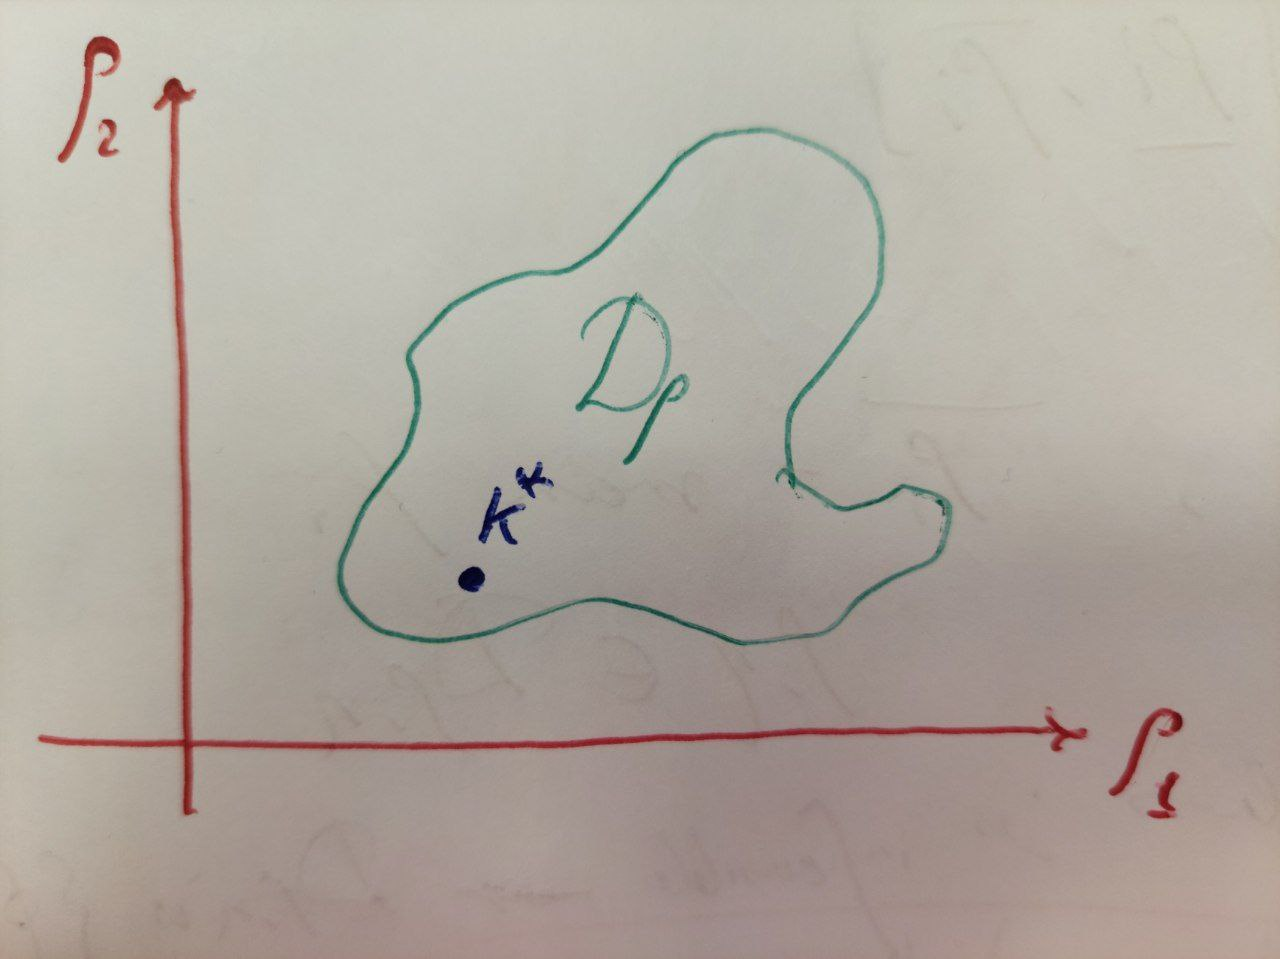
\includegraphics[width=0.65\textwidth]{d-rho.jpg}
    \caption{Feedback control system to be designed compared with the
 reference model $M(q^{-1})$}
 \end{figure}


\subsubsection{Result 8}:
Since we don't know $K^{*}$, if we assume that $K^{*} \in \mathcal{D}_\rho$, the worst-case estimation of $K^{*}$ is going to be for a K on the boundary of $\mathcal{D}$ with the largest distance, so we choose $K$ to be $K(\rho^c,q^{-1})$, where
\[
\rho^c = \arg \min_{\rho \in \mathbb{R}^{\text{length of $\rho$}}} \max_{\rho' \in \mathcal{D}_\rho} \|\rho - \rho'\|_\infty
\]

considering $l_\infty$ for our cost function, $\rho^c$ becomes the Chebyshev center of the FCPS.

\subsubsection{Result 9}:
It possible that the Chebyshev center in the $l_\infty$ norm is given by:
\[
\rho^c = \frac{\underline{\rho}+\overline{\rho}}{2}
\]
Since in $l_\infty$ we are considering a box around our $\mathcal{D}$ so the center of this box becomes the mean of the CPUIs.

Now, the procedure for the controller class is as follows. First, a first order model is chosen, then if it weren't feasible, the degree is increased, until we find a feasible solution.


\section{Stability Guarantee in Set-Membership Direct Data-Driven Control}

Considering DDDC, if M and the selected controller class are ”appropriate”, a solution exists.
The DDDC procedure leads to a controller built using the central estimate $\rho^c$
\[
K^c \equiv K(q^{-1},\rho^c)
\]

It is possible that the controller that is obtained in this manner, from the SM Identification does not make the closed-loop system stable.

The fact that we have noise in the data makes the problem of determining the stability harder. If we had noise free data, we could estimate perfectly the plant, and checking the stability would have been just checking basic stability criterion for our matrix transfer function.

The noise creates a phenomenon that we obtain an infinite number of models for our plant, so we have to check the stability of all of those systems. For doing so, we have to consider the worst case inside the set.



\subsection{problem setting}

According to the DDDC frmework, stability must be established in the following conditions.
\begin{itemize}
    \item The plant $P$ is known; we assume that the order of the plant is less than or equal to a given integer $n_p$.
    \item The controller $K^c$ has been designed and is fixed.
    \item A set of input-output data $\{r_t,\tilde{y}_t)\}$ collected on the plant is available. The output samples are corrupted by noise according to:
    \[
    \tilde{y}_t = y_t + \eta_t, \hspace{0.5cm} |\eta_t|\leq \Delta_\eta, \hspace{0.5cm} t=1,\,2,\,\cdots,\,N
    \]
\end{itemize}

Uncertainty on the data makes the problem of establishing stability harder. Stability must be ensured for all allowed realizations of the noise within the specified
bound.\\

Intuition: the noise induces uncertainty on the available information.
More uncertainty means harder to achieve stability.

\subsection{$H_\infty$-norm}
$H_\infty$ in the discrete-time domain is defined as follows:
\[
\|G(z)\|_\infty  \sup\limits_{\omega \in [0,\,2\pi]} |G(e^{i\omega})|
\]
\begin{factbox}
Here, we should have an idea about the $H_\infty$, the I studied it in the modern design of control system.\\

The physical intuition about this norm is that, it gives the maximum amplification of the energy of the input that your provide to a system.
\end{factbox}

\subsection{Small-gain theorem}
Almost all the results about the robustness in control theory is based on this theorem. This theory says if two systems $S1$ and $S2$ are connected as the following figure. 

\textbf{Theorem}: Suppose subsystems $S1$ and $S2$ are stable. Then, the interconnection of these two subsystem shown in the figure is \textbf{well-posed} and \textbf{internally stable} if and only if 
\[
\|S_1S_2\|_\infty < 1
\]
It is called in this way because of the previous argument about the energy amplification interpretation of $H_\infty$ norm. 
 \begin{figure}[H]
    \centering
    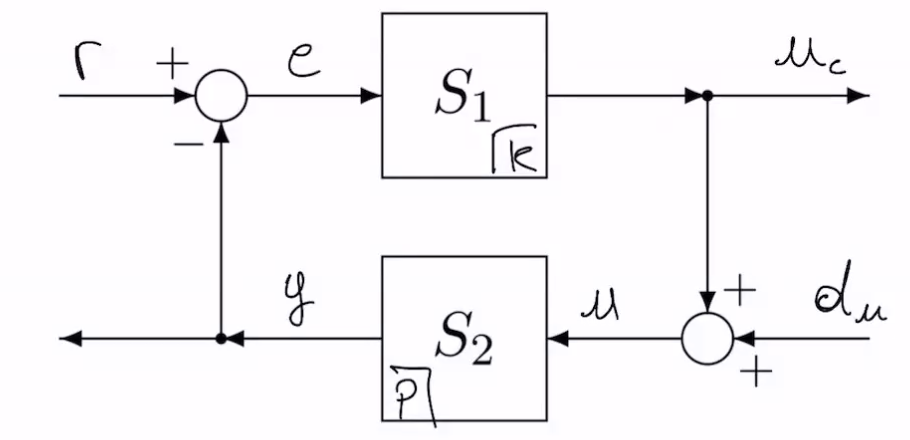
\includegraphics[width=0.4\textwidth]{interconnection-0.png}
    \caption{Inter-connection of two systems; here, S1 is considered as the controller and S2 is considered as the plant to be controlled.}
 \end{figure}


\begin{example}[Example]
Consider an unknown plant $P$. Let $P_n$ be a nominal description of the plant and $W_P$ a description of its uncertainty.\\
Assume that the model belongs to a class of multiplicative uncertainty model as follows:
\[
\{P: P = P_n (1 + W_P \Delta(z)),\,\,\|\Delta\|_\infty <1 \}
\]
Here, $P_n$ and $W_P$ are supposed to be known. \\

Now, we use the small-gain theorem. Considering the feedback control system, we consider $\Delta$ as our subsystem $S1$. 
 \begin{figure}[H]
    \centering
    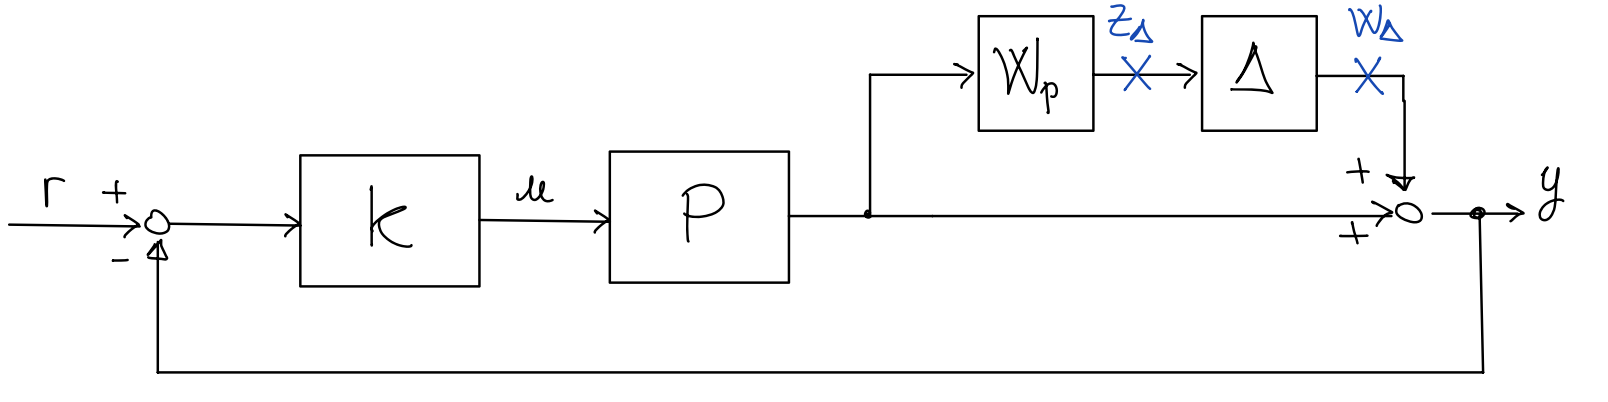
\includegraphics[width=0.75\textwidth]{small-gain-example.png}
    \caption{Block diagram of the feedback control system with uncertainty on the plant; in the discussion of indirect data drive design of controllers.}
 \end{figure}
 \[
 S1 \equiv \:\:\:\: S2 \equiv G_{w_\Delta z_\Delta} = \frac{-KP_nW_p}{1+KP_n}
 \]
 Here, $S1$ and $W_p$ is stable by assumption. Then, we should study the stability of $S2$. $S2$ is the multiplication of
 \[
 S2 = -T_n*W_p
 \]
 where
 \[
 T_n = \frac{KP_n}{1 + K P_n}
 \]
 and $T_n$ is stable if $K$ stabilizes the nominal plant.
 
 Small-gain theorem implies that:
 \[
 1 > \|S1S2\|_\infty = \|\Delta\frac{-KP_nW_P}{1 + KP_n}\|_\infty
 \]
 and adopting sum-multiplicativity property of induced norms. Induced norm is the norm defined by the worst case ratio between two norms in two different space. Since a system is an object which maps signals into signals, we can consider it as an operator between the space of signals. And if we define the norm of a signal as the energy of that signal, $H_\infty$ is the induced norm from the space of bounded energy signals.
 \[
 \|\Delta\frac{-KP_nW_P}{1 + KP_n}\|_\infty > \|\Delta\|_\infty \|\Delta\frac{KP_nW_P}{1 + KP_n}\|_\infty
 \]
 Since we know that $\|\Delta\|_\infty<1$ we obtain that 
 \[
 \|\frac{KP_nW_P}{1 + KP_n}\|_\infty < 1
 \]
 
\end{example}
\begin{example}
which means if 
\[
 \|\frac{KP_nW_P}{1 + KP_n}\|_\infty < 1
\]
the interconnection of the two systems is going to be stable two.
\end{example}


The previous example was about robust stability of a system, and, in general, any attempt to describe the uncertainty around a nominal plant inevitably leads to \textbf{indirect data-driven control}. However, in the connection of DDDC, the plant is unknown.\\

To circumvent this problem, We consider a \textbf{nominal feedback control system} with our \textbf{ideal controller}, and we consider \textbf{the uncertainty} resulting from the noisy data as a \textbf{distance between actual and ideal controller}.\\

 \begin{figure}[H]
    \centering
    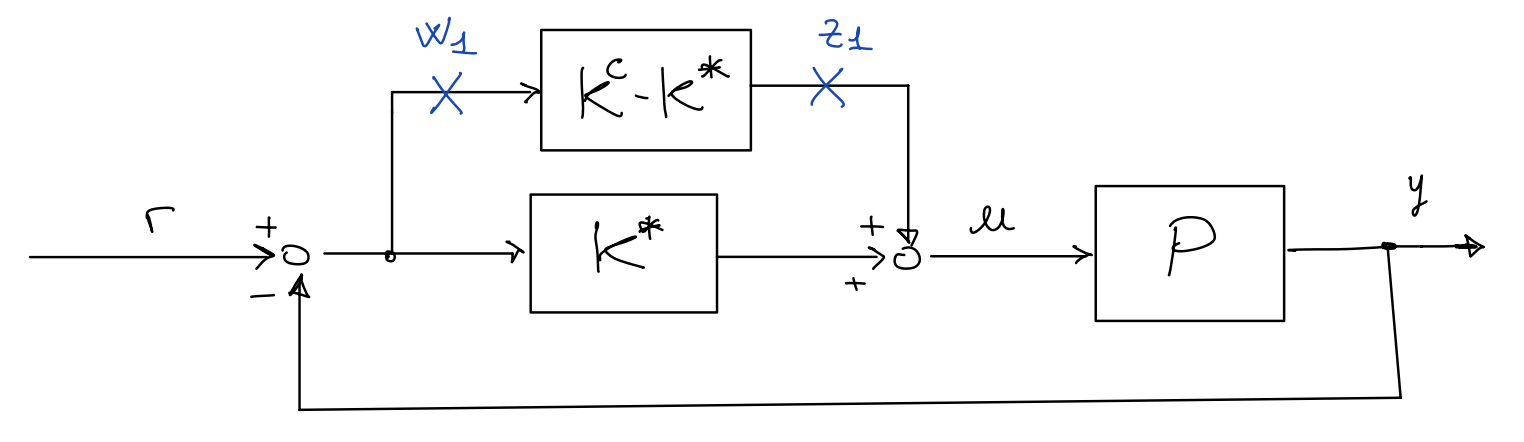
\includegraphics[width=0.75\textwidth]{small-gain-dddc.png}
    \caption{Block diagram of the feedback control system with uncertainty on the controller; this is in the context of DDDC.}
 \end{figure}

As it was discussed, $K^{*}$ is the ideal controller and the uncertainty is the distance of the ideal controller from the central controller $K^{c}$. Therefore,

\[
S1 \equiv K^{c} - K^{*} \:\:\:\: S2 \equiv \frac{-P}{1+K^{*}P} 
\]

Now consider the following theorem:\\

\textbf{Small-gain theorem in DDDC}:\\
Let
\[
\Delta(z) = M(z) - K^{c}P(z)(1-M(z))
\]
The controller $K^{c}$ stabilizes the plan $P$ if the following assumptions are satisfied:
\begin{itemize}
    \item The ideal controller $K^{*} = \frac{M}{P(1-M)}$ stabilizes the plant
    \item $\Delta(z)$ is stable
    \item $\|\Delta\|_\infty<1 $
\end{itemize}

So first, we have to show that our subsystems are stable.\\

$S2$ is the transfer function between $u$ and $y$ in the nominal system. Then, $S2$ is stable if the nominal system is stable, which means $K^{*}$ stabilizes the plant, that in turn is \textbf{our first assumption.}\\

Now, $S1$ should be stable. since $S2$ is stable then $S1$ is stable if and only if $S1S2$ is stable.\\


Let us evaluate $S1S2$
\[
S1S2 = (K^{c} - K^{*})\frac{-P}{1+K^{*}P} = \frac{K^{*}P}{1+K^{*}P} - \frac{K^{c}P}{1+K^{*}P} 
\]
It can be notices that the first term is the definition of our ideal sensitivity function and we can pull out an ideal sensitivity function from the second term.
\[
M = T^{*} = \frac{K^{*}P}{1+K^{*}P}
\]
\[
S^{*} = 1 - M = \frac{1}{1+ K^{*}P}
\]
Now, by substituting these two in our equation, the ideal controller is no longer needed to check the stability. By rewriting we obtain:
\[
M - K^{c}P(1-M)
\]
Which is what we considered $\Delta(z)$ in the description of our theorem.

$S1$ is stable if and only if $S1S2$ is stable and if and only if $\Delta$ is stable. \textbf{We consider this as our second assumption.}\\

Finally, 
\[
\|S1S2\|_\infty = \|\Delta\|_\infty < 1
\]
and this is our \textbf{assumption three}.

At this point, it is true that we eleminated $K^{*}$, but still we have the description of the plant in our theorem, which is not known in this context.


Regarding the first assumption, The ideal controller $K^{*} = \frac{M}{P(1-M)}$ stabilizes the plant \textbf{if and only if} $M$ is stable and no unstable cancellations occur, discussed in the previous section.\\
Now, we focus our attention on the second and the third assumption, which is we have to ensure that $\Delta = M - K^{c}P(1-M)$ is stable. To make sure that $Delta$ is stable we should make sure that its two terms are stable. $M$ is stable, since we want the final plant to be stable. $P$ is considered to be stable; otherwise, we would not be able to perform the experiment. $K^{c}$ is stable. Then, this condition is automatically satisfied. \\

Nevertheless, in practice, stability is not the only requirement. Most often, zero steady-error is also require, and in order to assure that, we require integrators, which make the controller unstable, and we cannot make the reasoning we just made. \\

Then we have our second sufficient condition. That is, $\Delta$ is stable if $M$ and $P$ are stable - the same reasoning as before holds - and if $K^{c}$ is \textbf{unstable only due to poles in} $z = 1$, our \textbf{loop function} $\frac{M}{1-M}$ have the same number of poles in $z = 1$.



















